\documentclass{article}
\renewcommand{\familydefault}{\sfdefault}
\usepackage{amsmath}
\usepackage{tikz}
\usetikzlibrary{positioning,arrows.meta,calc}
\pagestyle{empty}
\definecolor{enc}{RGB}{214,234,240}
\definecolor{encb}{RGB}{58,128,150}
\definecolor{cheap}{RGB}{226,239,220}
\definecolor{cheapb}{RGB}{88,140,72}
\definecolor{dec}{RGB}{252,228,214}
\definecolor{decb}{RGB}{196,110,60}
\definecolor{llm}{RGB}{233,224,244}
\definecolor{llmb}{RGB}{120,90,160}
\definecolor{store}{RGB}{222,232,250}
\newlength{\gap}\setlength{\gap}{1.0cm}  % one length for every horizontal arrow
\newsavebox{\fig}
\begin{document}
\sbox{\fig}{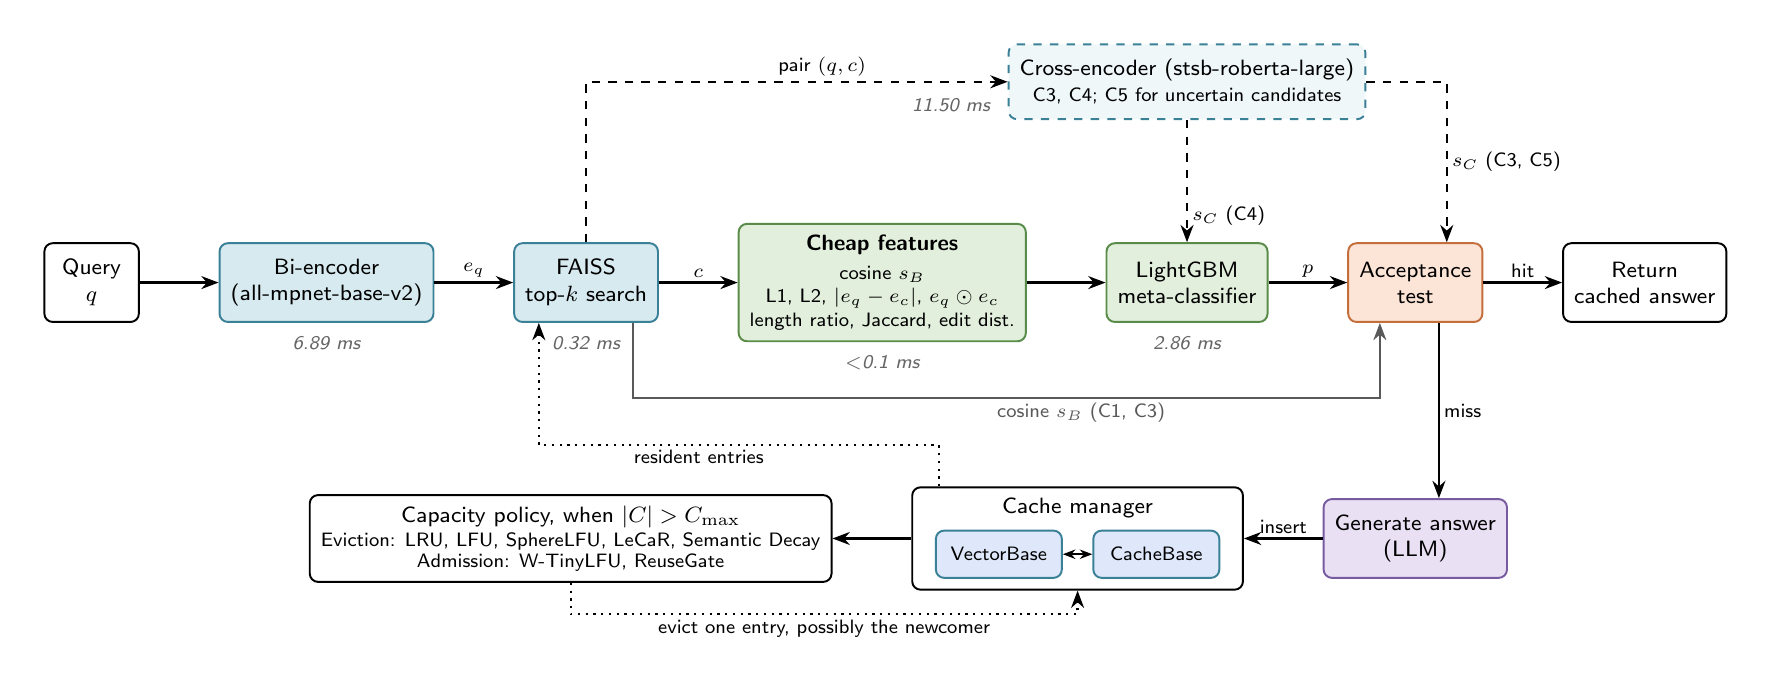
\begin{tikzpicture}[
  box/.style={draw, rounded corners=3pt, line width=0.7pt, align=center, font=\footnotesize, inner sep=4pt, minimum height=1.0cm},
  cost/.style={font=\scriptsize\itshape, text=black!60},
  arr/.style={-{Stealth[length=2.2mm]}, line width=0.8pt},
  darr/.style={-{Stealth[length=2.2mm]}, line width=0.8pt, dashed},
  lab/.style={font=\scriptsize, inner sep=1.5pt},
  node distance=\gap]

% ---------------- decision path ----------------
\node[box, minimum width=1.2cm] (q) {Query\\$q$};
\node[box, fill=enc, draw=encb, right=of q] (bi) {Bi-encoder\\(all-mpnet-base-v2)};
\node[box, fill=enc, draw=encb, right=of bi] (faiss) {FAISS\\top-$k$ search};
\node[box, fill=cheap, draw=cheapb, minimum height=1.45cm, right=of faiss] (feat)
  {\textbf{Cheap features}\\[1pt]\scriptsize cosine $s_B$\\[-1pt]\scriptsize L1, L2, $|e_q-e_c|$, $e_q\odot e_c$\\[-1pt]\scriptsize length ratio, Jaccard, edit dist.};
\node[box, fill=cheap, draw=cheapb, right=of feat] (lgb) {LightGBM\\meta-classifier};
\node[box, fill=dec, draw=decb, right=of lgb] (acc) {Acceptance\\test};
\node[box, right=of acc] (ret) {Return\\cached answer};

\node[cost, anchor=north] at ($(bi.south)+(0,-0.05)$) {6.89 ms};
\node[cost, anchor=north] at ($(faiss.south)+(0,-0.05)$) {0.32 ms};
\node[cost, anchor=north] at ($(feat.south)+(0,-0.05)$) {$<$0.1 ms};
\node[cost, anchor=north] at ($(lgb.south)+(0,-0.05)$) {2.86 ms};

\draw[arr] (q) -- (bi);
\draw[arr] (bi) -- node[lab, above]{$e_q$} (faiss);
\draw[arr] (faiss) -- node[lab, above]{$c$} (feat);
\draw[arr] (feat) -- (lgb);
\draw[arr] (lgb) -- node[lab, above]{$p$} (acc);
\draw[arr] (acc) -- node[lab, above]{hit} (ret);

% cross-encoder (dashed): C3 and C4, and C5 for uncertain candidates
\node[box, dashed, fill=enc!40, draw=encb, minimum height=0.95cm] (ce) at ($(lgb)+(0,2.55)$)
  {Cross-encoder (stsb-roberta-large)\\\scriptsize C3, C4; C5 for uncertain candidates};
\node[cost, anchor=east] at ($(ce.west)+(-0.1,-0.3)$) {11.50 ms};
\draw[darr] (faiss.north) |- node[lab, pos=0.78, above]{pair $(q,c)$} (ce.west);
\draw[darr] (ce.south) -- node[lab, right, pos=0.78]{$s_C$ (C4)} (lgb.north);
\draw[darr] (ce.east) -| node[lab, pos=0.75, right]{$s_C$ (C3, C5)} ($(acc.north)+(0.4,0)$);
\coordinate (sb) at ($(faiss.south)+(0,-0.95)$);
\coordinate (s0) at ($(faiss.south)+(0.6,0)$);
\draw[arr, black!65] (s0) -- (s0 |- sb) -| node[lab, pos=0.3, below]{cosine $s_B$ (C1, C3)} ($(acc.south)+(-0.45,0)$);

% ---------------- miss path ----------------
\node[box, fill=llm, draw=llmb] (gen) at ($(acc)+(0,-3.25)$) {Generate answer\\(LLM)};
\draw[arr] ($(acc.south)+(0.3,0)$) -- node[lab, right]{miss} ($(gen.north)+(0.3,0)$);
\node[box, minimum width=4.2cm, minimum height=1.3cm, left=of gen] (cm) {};
\node[font=\footnotesize, anchor=north] at ($(cm.north)+(0,-0.02)$) {Cache manager};
\node[box, fill=store, draw=encb, minimum width=1.6cm, minimum height=0.6cm, font=\scriptsize] (vb) at ($(cm.center)+(-1.0,-0.2)$) {VectorBase};
\node[box, fill=store, draw=encb, minimum width=1.6cm, minimum height=0.6cm, font=\scriptsize] (cb) at ($(cm.center)+(1.0,-0.2)$) {CacheBase};
\draw[{Stealth[length=1.6mm]}-{Stealth[length=1.6mm]}, line width=0.6pt] (vb) -- (cb);
\draw[arr] (gen) -- node[lab, above]{insert} (cm);
\coordinate (rm) at ($(faiss.south)+(0,-1.55)$);
\coordinate (r0) at ($(cm.north west)+(0.35,0)$);
\draw[arr, dotted] (r0) -- (r0 |- rm) -| node[lab, pos=0.3, below]{resident entries} ($(faiss.south)+(-0.6,0)$);
\node[box, left=of cm] (ev) {Capacity policy, when $|C|>C_{\max}$\\[-1pt]\scriptsize Eviction: LRU, LFU, SphereLFU, LeCaR, Semantic Decay\\[-2pt]\scriptsize Admission: W-TinyLFU, ReuseGate};
\draw[arr] (cm) -- (ev);
\draw[arr, dotted] (ev.south) -- ++(0,-0.4) -| node[lab, pos=0.25, below]{evict one entry, possibly the newcomer} (cm.south);

% margin
\path ([shift={(-2mm,-2mm)}]current bounding box.south west) rectangle ([shift={(2mm,2mm)}]current bounding box.north east);
\end{tikzpicture}}%
\pdfpagewidth=\wd\fig \pdfpageheight=\dimexpr\ht\fig+\dp\fig\relax
\hoffset=-1in \voffset=-1in \oddsidemargin=0pt \topmargin=0pt \headheight=0pt \headsep=0pt
\textwidth=\wd\fig \parindent=0pt
\noindent\usebox{\fig}
\end{document}
